\chapter{Specification} \label{specifications}

\section{Functional Description}\label{functional-description}

The AHB-Lite Timer IP is a fully parameterised Timer-tick core,
featuring a single AHB-Lite Slave interface and a single multiplexed
Interrupt output signal.

The Timer IP is intended to generate CPU interrupts at regular time
intervals, for timed events such as time keeping, task/context switches,
and sleep().

The number of timers and Address \& Data width of the AHB-Lite interface
are specified via parameters defined at compile time.

The time base of the timers is common to all timers and defined at
runtime by writing to the PRESCALER register. Individual timer alarms
may then set via the TIMECMP{[}n{]} registers. All timers are
permanently enabled however a separate IENABLE register allows any
triggered counter output to be masked.

The user may determine both the status of the TIMERS including which
timer has generated an interrupt via a read operation to the AHB-Lite
interface.

\begin{figure}[tbh]
	\centering
	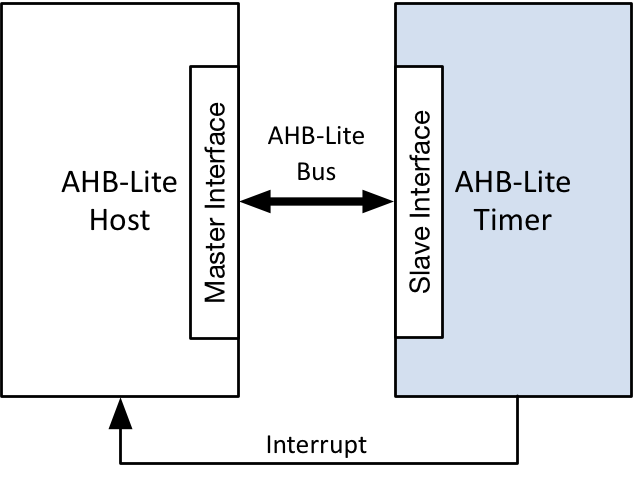
\includegraphics{assets/img/AHB-Lite-Timer-sys.png}
	\caption{AHB-Lite Timer System Diagram}
	\label{fig:ahb-lite-timer-sys}
\end{figure}
